\begin{frame}[c]{}

\centering
\huge
Lectures 11:\\
Beyond AutoML: Algorithm Configuration and Control
\end{frame}
%----------------------------------------------------------------------
\begin{frame}[c]{Where are we? The big picture}

\begin{itemize}
	\item Introduction
	\item Background
	\begin{itemize}
		\item Design spaces in ML
		\item Evaluation and visualization
	\end{itemize}
	\item Hyperparameter optimization (HPO)
	\begin{itemize}
		\item Bayesian optimization
		\item Other black-box techniques
		\item More details on Gaussian processes
	\end{itemize}
	\item Pentecost (Holiday) -- no lecture
	\item Architecture search I + II
	\item Meta-Learning I + II
	\item[$\to$] Beyond AutoML: algorithm configuration and control
	\item Project announcement and closing
\end{itemize}

\end{frame}
%----------------------------------------------------------------------

%----------------------------------------------------------------------
\begin{frame}[c]{Learning Goals}

After this lecture, you will be able to \ldots

\begin{itemize}
	\item define the \alert{algorithm configuration problem}
	\item discuss \alert{differences} between HPO and algorithm configuration
	\item explain the \alert{components of SMAC} to combine Bayesian Optimization across instances
	\item define and give examples for the \alert{algorithm control problem}
	\item list some \alert{further topics} related AutoML and algorithm configuration
\end{itemize}

\end{frame}
%-----------------------------------------------------------------------
%----------------------------------------------------------------------
\begin{frame}[c]{Further Material}

There is one recent tutorials on algorithm configuration:

\begin{itemize}
	\item ICML'19: Frank Hutter and Kevin Leyton-Brown on\\
	"Algorithm configuration: learning in the space of algorithm designs"\\
	\footnotesize{\url{https://www.facebook.com/icml.imls/videos/vb.118896271958230/2044426569187107/}}
\end{itemize}


\end{frame}
%-----------------------------------------------------------------------
\section{Algorithm Configuration}
%----------------------------------------------------------------------
\begin{frame}[c]{Generalization of HPO}

\begin{itemize}
	\item hyperparameter optimization (HPO) is not limited to ML
	\pause
	\item in fact, you can optimize the performance of any algorithm by means of HPO if
	\begin{enumerate}
		\item the algorithm at hand has parameters that influence its performance
		\item you care about the empirical performance of an algorithm
	\end{enumerate}
	\pause
 	\smallskip
 	\item a limitation of HPO is that we assume that we care only about a single task (i.e., dataset or input to the algorithm)
 	\smallskip
 	\item[$\leadsto$] \alert{Can we find an algorithm's configuration that performs well and robustly across a set of tasks?}
 	\begin{itemize}
 		\item An hyperparameter configuration for a set of datasets
 		\item A parameter configuration of a SAT solver for a set of SAT instances
 		\item A parameter configuration of a AI planning solver for a set of planning problems
 		\item \ldots
 	\end{itemize}
 	\item[$\leadsto$] \alert{Algorithm configuration}
\end{itemize}


\end{frame}
%----------------------------------------------------------------------
%----------------------------------------------------------------------
\begin{frame}[c]{Algorithm Configuration Visualized}

\centering
\scalebox{0.5}{
	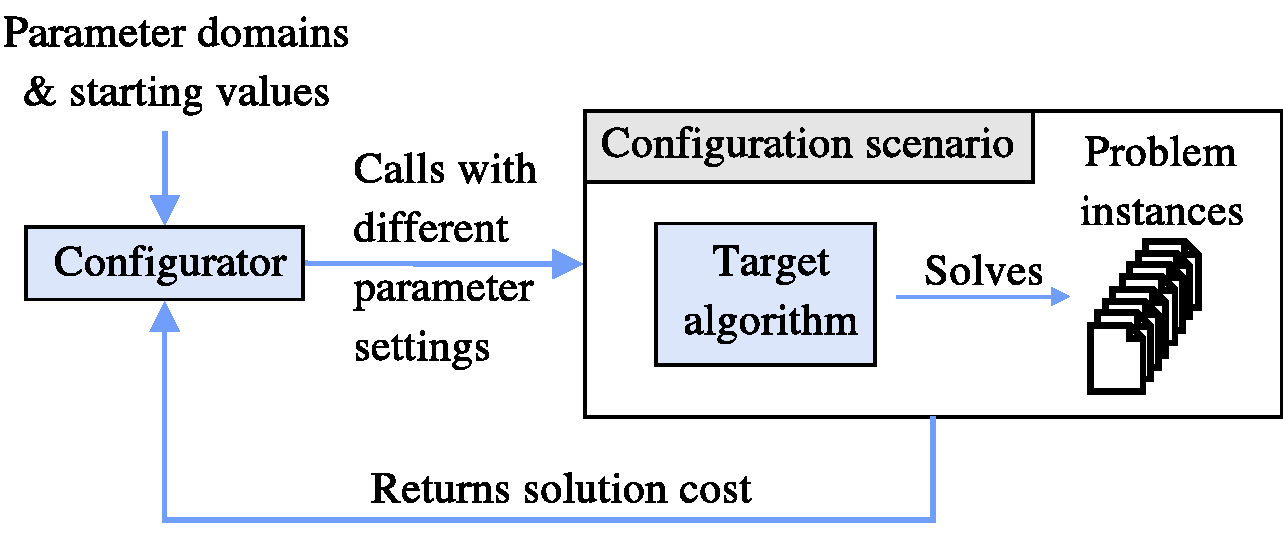
\includegraphics{images/Configuration-Process.pdf}
}

\end{frame}
%-----------------------------------------------------------------------
%----------------------------------------------------------------------
\begin{frame}[c]{Algorithm Configuration -- in More Detail}

\bigskip

\centering
\scalebox{0.75}{
	\tikzstyle{activity}=[rectangle, draw=black, rounded corners, text centered, text width=8em, fill=white, drop shadow]
\tikzstyle{wideactivity}=[rectangle, draw=black, rounded corners, text centered, text width=10em, fill=white, drop shadow]
\tikzstyle{data}=[rectangle, draw=black, text centered, fill=black!10, text width=8em, drop shadow]
\tikzstyle{myarrow}=[->, thick]
\begin{tikzpicture}[node distance=5cm,thick]
	%PreProcessing
	%\node (Algo) [data] {Algorithm $A$};
	\node (Data) [data] {Instances $\insts$};
	\node (CS) [data, right of=Data, xshift=-0.5cm] {Algorithm $\algo$ and\\ its Configuration\\ Space $\pcs$};
	\node (Select) [activity, below of=Data, node distance=2.0cm] {Select $\conf \in \pcs$\\ and $\inst \in \insts$};
	\node (Run) [wideactivity, right of=Select, xshift=-0.5cm] {Run $\algo(\conf)$ on $\inst$ to measure $c(\conf,\inst)$};
	%\node (Return) [activity, right of=Run, text width=9em] {Return Performance\\ of $A(c)$ on $I'$}; 
	%\node (Data) [data, left of=Select] {Instances $I$};	
	\node (Result) [activity, right of=Run, node distance=4.6cm] {Returns Best\\ Configuration $\hat{\conf}$}; 
	
	\draw[myarrow] (Data) -- ($(Select)+(-0.0,+0.8)$);
	\draw[myarrow] (CS) -- ($(Run)+(-0.0,+0.8)$);
	%\draw[myarrow] (Data) -- ($(Select)+(-2.1,+0.0)$);
	
	%\draw[thick, dashed] (Algo) -- (CS);
	\draw[myarrow] ($(Run.east)+(0.25,0)$) -- (Result);
	\draw[myarrow] (Select) -- (Run);
	%\draw[myarrow] (Run) -- (Return);
	\draw[myarrow] (Run.south) |- ++(0.0,-0.8)  node[above, xshift=-2.2cm] {Return Cost} -| (Select.south);
	
	\begin{pgfonlayer}{background}
    
        % Configuration Process
    	\path (Select -| Select.west)+(-0.25,0.85) node (resUL) {};
    	\path (Run.east |- Run.south)+(0.25,-1.3) node(resBR) {};
    	\path [rounded corners, draw=black!60, dashed] (resUL) rectangle (resBR);
		\path (Run.east |- Run.south)+(-1.5,-1.1) node [text=black!60] {Configuration Task};
    	
    \end{pgfonlayer}
	
\end{tikzpicture}

}

\bigskip

\begin{block}{Definition}
	Given a parameterized algorithm $\algo$ with possible parameter settings $\confs$, \pause 
	a set of training problem instances $\insts$, \pause 
	and a cost metric $c: \confs \times \insts \rightarrow \perf$, \pause 
	the algorithm configuration problem is 
	to \alert{find a parameter configuration $\conf^* \in \confs$ 
		that minimizes $c$ across the instances in $\insts$}.
\end{block}

\end{frame}
%-----------------------------------------------------------------------


%----------------------------------------------------------------------
\begin{frame}[c]{Algorithm Configuration -- Full Formal Definition}

\begin{block}{Definition}
An instance of the algorithm configuration problem
is a 5-tuple $(\algo, \pcs, \instD, \cutoff, c)$ where:
\begin{itemize}
	\item $\algo$ is a parameterized algorithm;
	\item $\pcs$ is the parameter configuration space of $\algo$;
	\item $\instD$ is a distribution over problem instances with domain $\insts$;
	\pause
	\item $\cutoff < \infty$ is a \alert{cutoff time}, after which each run of $\algo$ will be terminated if still running
	\pause
	\item $c: \confs \times \insts \rightarrow \mathds{R}$ is a function that
	measures the observed cost of running $\algo(\conf)$ on an instance $\inst \in
	\insts$ with cutoff time $\cutoff$ 
	%  \item $s$ is a statistical population parameter\\ (e.g., expectation, median,  or variance)
\end{itemize}
\pause
The cost of a candidate solution $\conf\in\confs$ is
%\begin{equation}
%\hat{\conf} \in \argmin_{\conf \in \pcs}
\alert{$f(\conf) = \mathds{E}_{\inst \sim \instD} (c(\conf,\inst))$}.\\
The goal is to find \alert{$\conf^* \in \argmin_{\conf \in \pcs} f(\conf)$}.
%\end{equation}

\end{block}

\end{frame}
%-----------------------------------------------------------------------

%----------------------------------------------------------------------
\begin{frame}[c]{Distribution of Instances}

We usually have a finite number of instances from a given application
\begin{itemize}
\item We want to do well on that type of instances
\item Future instances of this type should be solved well 
\end{itemize}

\pause
\bigskip

Like in machine learning
\begin{itemize}
\item We split the instances into a \alert{training set} and a \alert{test set}
\item We configure algorithms on the training instances
\item We only use the test instances afterwards
\begin{itemize}
\item[$\to$] unbiased estimate of generalization performance for unseen instances
\end{itemize}  
\end{itemize}


\end{frame}
%-----------------------------------------------------------------------
\begin{frame}[c]{Challenges of Algorithm Configuration}

\begin{itemize}
\item \alert{Structured high-dimensional parameter space}
\begin{itemize}
\item categorical vs. continuous parameters
\item conditionals between parameters
\end{itemize}
\pause
\medskip
\item \alert{Stochastic optimization}
\begin{itemize}
\item Randomized algorithms: optimization across various seeds
\item Distribution of benchmark instances (often wide range of hardness)
\item Subsumes so-called \emph{multi-armed bandit problem}
\end{itemize}
\pause
\medskip
\item \alert{Generalization across instances}
\begin{itemize}
	\item apply algorithm configuration to \alert{homogeneous} instance sets
	\item Instance sets can also be \alert{heterogeneous},\\i.e., no single configuration performs well on all instances\\ 
	\item[$\leadsto$] combination of algorithm configuration and selection
\end{itemize}

\end{itemize}

\pause
\medskip
$\leadsto$ Hyperparameter optimization is a subproblem of algorithm configuration

\end{frame}
%-----------------------------------------------------------------------


\section{SMAC: BO for Algorithm Configuration}

%-----------------------------------------------------------------------
\begin{frame}[c]{State-of-the-art Algorithm Configuration}

SMAC: Sequential Model-based Algorithm Configuration =

\begin{itemize}
	\item + Bayesian Optimization (instead of local search)
	\item + aggressive racing
	\item + adaptive capping (for optimizing runtime)
\end{itemize}

\end{frame}
%-----------------------------------------------------------------------
%-----------------------------------------------------------------------
\begin{frame}[c]{SMAC: Overview}
%\\\litw{Hutter et al. 2011}}

\LinesNotNumbered
\begin{algorithm}[H]
	\Input{%
		instance set $\insts$,
		Algorithm $\algo$ with configuration space $\confs$,
		Initial configuration $\conf_0$,
		performance metric $c$,
		Configuration budget $b$
	}
	\Output{best incumbent configuration $\hat{\conf}$}
	\BlankLine
	run history H $\leftarrow$ initial design based on $\conf_0$; \tcp*{H = $(\conf, \inst, c(\inst,\conf))_i$}
	\While{$b$ remains} {
		\pause
		$\epm \leftarrow$ train empirical performance model based on run history H;\\
		\pause
		$\confs_{challengers} \leftarrow$ select configurations based on $\epm$;\\
		\pause
		$\hat{\conf}$, H $\leftarrow$ intensify($\confs_{challengers}$, $\hat{\conf}$); \tcp*{racing and capping}
	}
	\pause
	\Return{$\hat{\conf}$}
	\caption{SMAC}
\end{algorithm}

\end{frame}
%-----------------------------------------------------------------

%-----------------------------------------------------------------------
\begin{frame}[c]{Comparisons on $N$ instances}

\begin{itemize}
	\item \alert{Basic(N)} uses a pretty basic comparison: \textit{better$_N(\conf', \conf)$}:
	\begin{itemize}
		\item Compare $\conf'$ and $\conf$ based on $N$ instances 
		\pause
		\item How does this relate to cross-validation? \hands
	\end{itemize}  
	
	\bigskip
	\pause
	\item Problem: How to set $N$? Problems of large $N$? Small $N$? \hands
	\pause
	\begin{itemize}
		\item Problem of large $N$: evaluations are slow
		\item Problem of small $N$: overfitting to a small set of instances
		\item[$\leadsto$] Tradeoff: Choose $N$ of moderate size 
	\end{itemize}
	
\end{itemize}
\end{frame}
%-----------------------------------------------------------------------


%-----------------------------------------------------------------------
\begin{frame}[c]{Comparisons on $N$ instances}


Question: \alert{Which} $N$ instances should we use? \hands
\begin{enumerate}
\item $N$ different instances for each configuration
\item The same set of $N$ instances for the entire run
\end{enumerate}

\bigskip
\pause
Answer: the same $N$ instances, so that we compare apples with apples
\begin{itemize}
\item[] (but: using the same instances can also yield overtuning) 
\end{itemize}
\bigskip


If we sampled different instances for each configuration:
\begin{itemize}
\item Some configurations would randomly get easier instances
\item Those configurations would look better than they really are
\end{itemize}

\end{frame}
%-----------------------------------------------------------------------



%-----------------------------------------------------------------------
\begin{frame}[c]{Comparisons on $N$ instances}

Question: For randomized algorithms, how should we set the seeds? \hands
\begin{enumerate}
\item Sample a new seed for each algorithm run
\item Fix the seeds together with the instances
\end{enumerate}
\bigskip
\pause
Answer: just like for instances, fix them to compare apples to apples

\bigskip
\pause
In summary, for each run of Basic(N): \\pick $N$ (instance, seed) pairs and use them for evaluating each $\conf$.\\
\pause
(Different Basic(N) runs can use different instances and seeds.)

\end{frame}
%-----------------------------------------------------------------------


%-----------------------------------------------------------------------
\begin{frame}[c]{The concept of overtuning}

Very related to overfitting in machine learning 
\begin{itemize}
\item Performance improves on the training set
\item Performance does not improve on the test set, and may even degrade
\end{itemize}	

\pause
\medskip

More pronounced for more heterogeneous benchmark sets 
\begin{itemize}
\item But it even happens for very homogeneous sets
\item Indeed, one can even overfit on a single instance, to the \alert{seeds} used for training 
\end{itemize}	

\end{frame}
%-----------------------------------------------------------------------

%-----------------------------------------------------------------------
\begin{frame}[fragile]{Overtuning Visualized}

\begin{itemize}
\item Example: minimizing SLS solver runlengths for a single SAT instance
\item \alert{Training cost}, e.g., with N=100:\\average runlengths across 100 runs with different seeds
\item \alert{Test cost} of $\hat{\conf}$ here based on 1000 new seeds 
\end{itemize}	

\pause


\begin{center}
\only<2>{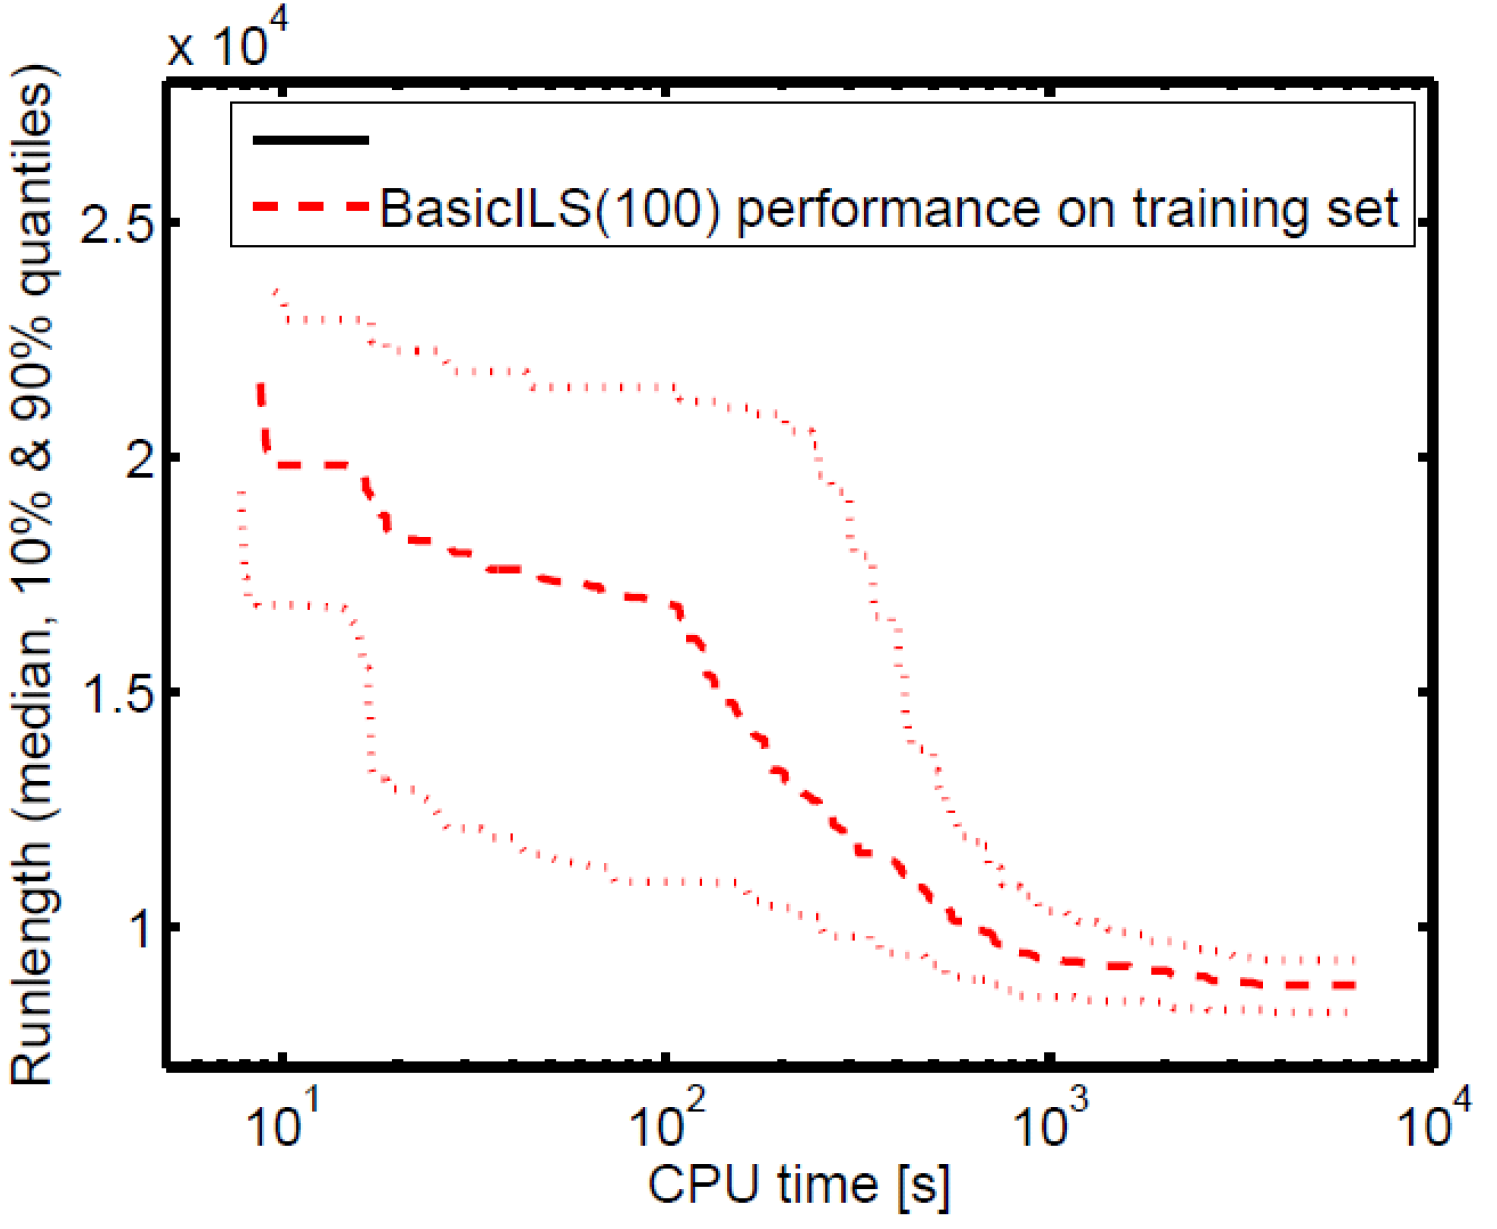
\includegraphics[scale=0.13]{images/basicils100_training.png}}
\only<3>{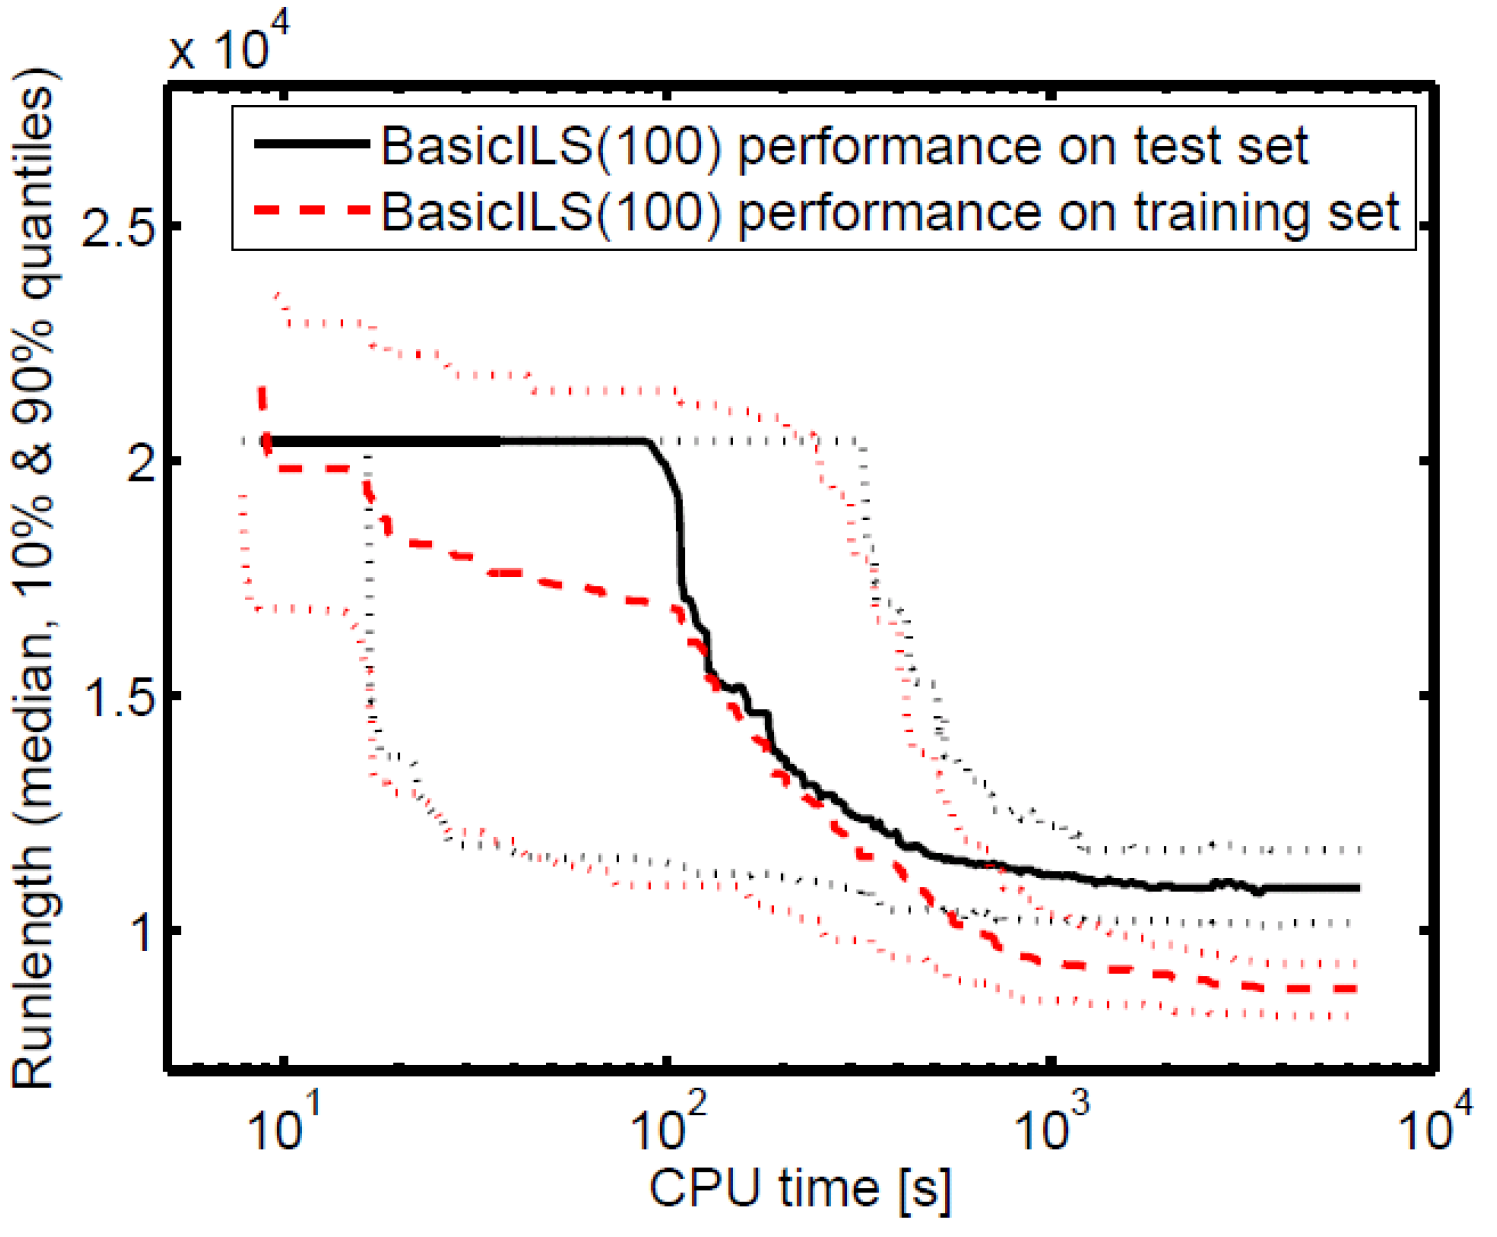
\includegraphics[scale=0.13]{images/basicils100_training_and_test.png}}
\end{center}


\end{frame}
%-----------------------------------------------------------------------

%-----------------------------------------------------------------------
\begin{frame}[fragile]{Basic(N) Test Results with Various N}

\begin{itemize}
\item Example: minimizing SLS solver runlengths for a single SAT instance
\item \alert{Training cost}, e.g., with N=?:\\average runlengths across N runs with different seeds
\item \alert{Test cost} of $\hat{\conf}$ here based on 1000 new seeds 
\end{itemize}	

\pause

\begin{multicols}{2}
\begin{center}
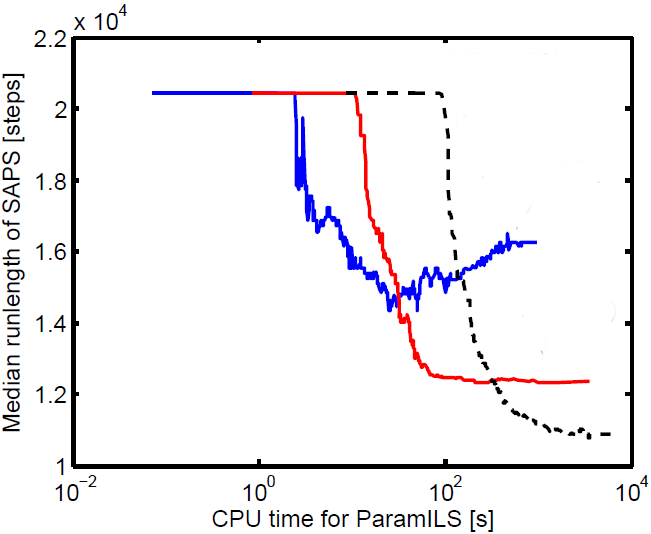
\includegraphics[scale=0.2]{images/basicils_unlabled.png}
\end{center}
\columnbreak{}
\pause
Which of these results corresponds to $N=1$, $N=10$, and $N=100$?\\
\hands

\pause
\medskip

\begin{enumerate}
\item N=1: blue, N=10: red,\\ N=100 dashed black
\item N=1: dashed black,\\ N=10: red, N=100 blue
\end{enumerate}

\pause
Correct Answer: 1


\end{multicols}


\end{frame}
%-----------------------------------------------------------------------



%-----------------------------------------------------------------------
\begin{frame}[c,fragile]{Aggressive Racing (inspired by FocusedILS)}

Intuition: get the best of both worlds
\begin{itemize}
\item Perform more runs for good configurations
\begin{itemize}
\item[-] to avoid overtuning
\end{itemize}
\item Quickly reject poor configurations
\begin{itemize}
\item[-] to make progress more quickly
\end{itemize}
\end{itemize}

\pause
\medskip

\begin{block}{Definition: $N(\conf)$ and $c_N(\conf)$}
\alert{$N(\conf)$} denotes the number of runs executed for $\conf$ so far.\\
\alert{$\hat{c}_N(\conf)$} denotes the cost estimate of $\conf$ based on $N$ runs.
\end{block}

\pause
In the beginning: $N(\conf)=0$ for every configuration $\conf$

\end{frame}

%-----------------------------------------------------------------------



%-----------------------------------------------------------------------
\begin{frame}[c,fragile]{Aggressive Racing}


\begin{block}{Definition: domination}
\alert{$\conf_1$ dominates $\conf_2$} if 
\begin{itemize}
\item $N(\conf_1) \ge N(\conf_2)$ and 
\item $\hat{c}_{N(\conf_2)}(\conf_1) \le \hat{c}_{N(\conf_2)}(\conf_2)$.
\end{itemize}
I.e.: we have at least as many runs for $\conf_1$ and its cost is at least as low.
\end{block}

\pause

\begin{block}{\textit{better($\conf', \conf^*$)} in a nutshell}
\begin{itemize}
\item $\conf^*$ is the current configuration to beat (incumbent)
\pause
\item Perform runs of $\conf'$ until either
\begin{itemize}
\item $\conf^*$ dominates $\conf'$ $\leadsto$ reject $\conf'$, or
\item $\conf'$ dominates $\conf^*$ $\leadsto$ change current configuration $(\conf^* \leftarrow \conf')$
\end{itemize}
\pause	
\item Over time: perform extra runs of $\conf^*$ to gain more confidence in it
\end{itemize}
\end{block}

\end{frame}

%-----------------------------------------------------------------------


%-----------------------------------------------------------------------
\begin{frame}[c,fragile]{Toy Example}


\begin{itemize}
\item Let $\conf^*$ be the incumbent  (evaluated on $\pi_1, \pi_2, \pi_3$)
\item We'll look at challengers $\conf'$ and $\conf''$
\end{itemize}

\begin{center}
\begin{tabular}{l ccc}
& $\inst_1$ & $\inst_2$ & $\inst_3$ \\
\hline
$\conf^*$ 	& 3 		& 2			& 10	\onslide<2->\\
\hline
$\conf'$		& \onslide<3->{2}			& \onslide<4->{10} 		& \\
& 			& \onslide<5->{$\to$ reject, since $\hat{c}_2(\conf')=6 > \hat{c}_2(\conf^*)=2.5$} & \\
\hline
\onslide<6->{$\conf''$}		& \onslide<6->{3}			& \onslide<7->{1} 		& \onslide<8->{5}\\
\end{tabular}
\end{center}

\onslide<9->
\begin{itemize}
\item new incumbent: $\conf^* \leftarrow \conf''$
\item Perform an additional run for new $\conf^*$ to increase confidence over time
\end{itemize}


\end{frame}
%-----------------------------------------------------------------------


%-----------------------------------------------------------------------
\begin{frame}[fragile]{Racing achieves the best of both worlds}

Aggressive racing (aka FocusedILS): Fast progress and no overtuning

\begin{center}
Test performance\\
\only<1>{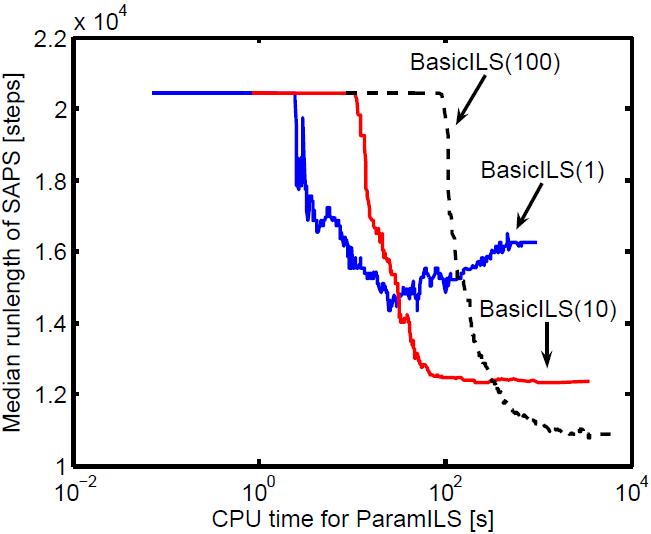
\includegraphics[scale=0.25]{images/basicils.png}}
\only<2>{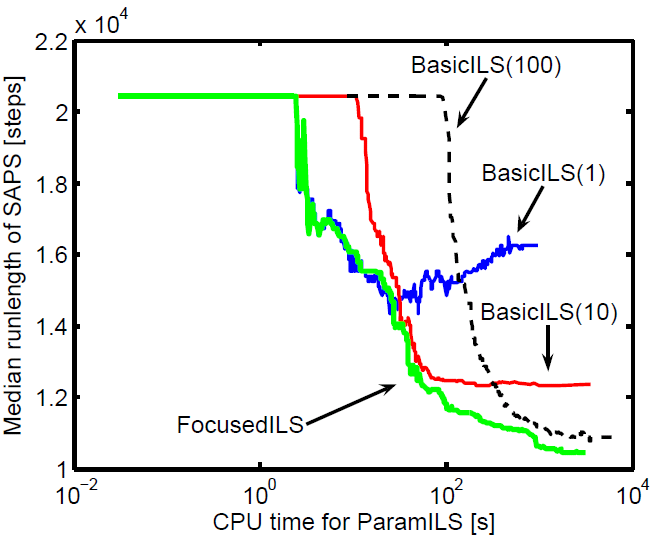
\includegraphics[scale=0.25]{images/focusedils.png}}
\end{center}

\end{frame}
%-----------------------------------------------------------------------

%-----------------------------------------------------------------------
\begin{frame}[c,fragile]{Adaptive capping}

\begin{itemize}
\item Assumptions
\begin{itemize} 
\item optimization of runtime
\item each configuration run has a time limit (e.g., $300$ sec)
\end{itemize}
\pause    

\item E.g., $\conf^*$ needed $1$ sec to solve $\inst_1$
\begin{itemize}
\item Do we need to run $\conf'$ for $300$ sec?
\item Terminate evaluation of $\conf'$ once guaranteed to be worse than $\conf^*$
\end{itemize}
\pause
\bigskip    
\item[$\leadsto$] To compare against $\conf^*$ based on $N$ runs,\\we can terminate evaluation of $\conf'$ after time $\sum_{i=1}^N c(\conf^*,\inst_i)$
\end{itemize}

\end{frame}
%-----------------------------------------------------------------------
%-----------------------------------------------------------------------
\begin{frame}[c,fragile]{Toy-Example: Adaptive capping}

runtime cutoff $\kappa = 300$, comparison based on 2 instances (using $\hat{c}_3$)

\begin{center}
\begin{tabular}{l cc}
& $\inst_1$ & $\inst_2$ \\
\hline
$\conf^*$ 	& 4 		& 2		\onslide<2->\\
\hline
\multicolumn{3}{l}{\emph{Without adaptive capping}}\\
$\conf'$		& \onslide<3->{3}			& \onslide<4->{300} 		\\
& 			&  \onslide<5->{$\to$ reject $\conf'$ (\alert{cost: 303})}\onslide<6->\\
\hline
\multicolumn{3}{l}{\onslide<6->{\emph{With adaptive capping}}}\\
$\conf'$\onslide<7->			& \onslide<7->{3}		& \onslide<8->{300} 	\\
& 					 \multicolumn{2}{l}{\onslide<9->$\to$ \alert{cut off} after $\kappa=4$ seconds, reject $\conf'$ (\alert{cost: 7})} \\
\hline
\end{tabular}
\end{center}

\medskip
\onslide<10-> 
{Note: To combine adaptive capping with BO, we need to impute the censored observations caused by adaptive capping.}


\end{frame}
%-----------------------------------------------------------------------
%-----------------------------------------------------------------------
\begin{frame}[c]{SMAC: Overview}
%\\\litw{Hutter et al. 2011}}

\LinesNotNumbered
\begin{algorithm}[H]
	\Input{%
		instance set $\insts$,
		Algorithm $\algo$ with configuration space $\confs$,
		Initial configuration $\conf_0$,
		performance metric $c$,
		Configuration budget $b$
	}
	\Output{best incumbent configuration $\hat{\conf}$}
	\BlankLine
	run history H $\leftarrow$ initial design based on $\conf_0$; \tcp*{H = $(\conf, \inst, c(\inst,\conf))_i$}
	\While{$b$ remains} {
		$\epm \leftarrow$ train empirical performance model based on run history H;\\
		$\confs_{challengers} \leftarrow$ select configurations based on $\epm$; \tcp*{BO with EI} 
		$\hat{\conf}$, H $\leftarrow$ intensify($\confs_{challengers}$, $\hat{\conf}$); \tcp*{racing and capping}
	}
	\Return{$\hat{\conf}$}
	\caption{SMAC}
\end{algorithm}

\end{frame}
%-----------------------------------------------------------------
\section{Teaching Evaluation}

\section{Algorithm Control}
%-----------------------------------------------------------------------
%----------------------------------------------------------------------
\begin{frame}[c]{Dynamic Heuristics}

\begin{itemize}
	\item Many heuristics in algorithms are dynamic and adaptive
	\begin{enumerate}
		\item the algorithm's behavior changes over time
		\item the algorithm's behavior changes based on internal statistics
	\end{enumerate}
	\medskip
	\item these heuristics might control other parameters of the algorithms
	\pause
	\smallskip
	\item example: learning rate schedules for training DNNs
	\begin{enumerate}
		\item exponential decaying learning rate: based on number of iterations, learning rate decreases
		\pause
		\item Reduce learning rate on plateaus: if the learning stagnates for some time, the learning rate is decreased by a factor
	\end{enumerate}
	\pause
	\item What examples for dynamic heuristics can you think of? \hands
	\pause
	\item other examples: restart probability of search, mutation rate of evolutionary algorithms, \ldots  
	
\end{itemize}

\end{frame}
%----------------------------------------------------------------------
%----------------------------------------------------------------------
\begin{frame}[c]{Parametrization of Learning Rate Schedules}

\begin{itemize}
\item How would we parameterize learning rate schedules?
\begin{enumerate}
	\item exponential decaying learning rate:
	\begin{itemize}
		\item initial learning rate
		\item minimal learning rate
		\item multiplicative factor
	\end{itemize}
	\pause
	\item Reduce learning rate on plateaus:
	\begin{itemize}
		\item patience (in number of epochs)
		\item patience threshold
		\item decreasing factor
		\item cool-down break (in number of epochs)
	\end{itemize}
\end{enumerate}
\pause
\medskip
\item[$\leadsto$] Many parameters only to control a single parameter (learning rate)
\pause   
\item Still not guaranteed that optimal setting of learning rate schedules will lead to optimal learning rate behavior
\begin{itemize}
	\item Learning rate schedules are only heuristics
\end{itemize}
\end{itemize}

\end{frame}
%----------------------------------------------------------------------
%----------------------------------------------------------------------
\begin{frame}[c]{Algorithm Control \litw{Biedenkapp et al. 2019}}

\begin{itemize}
	\item Goal: control a (set of) hyperparameter(s) during the run
	\item Problem can be defined as an MDP $\mdp\coloneqq(\states,\actions,\transitions,\rewards)$
	\begin{description}
		\item[State Space $\states$] At each time step $t$, internal state $s_t$ of the target algorihtm being controlled.
		\item[Action space $\actions$] Given a state $s_t$, the controller has to decide how to change the value $v\in\actions_h$
		of a hyperparameter $h$.
		\item[Transition Function $\transitions$] dynamics of the algorithm at hand transitioning from $s_t$ to $s_{t+1}$ by applying action $a_t$ with probability $t(s_t, a_t, s_{t+1})$
		\item[Reward $\rewards$] Either sparse reward at the end of the algorithm run or intermediate run quality estimate
		
	\end{description}
\end{itemize}

\pause

\vspace*{-0.5cm}            
\begin{align}
\policy^*(s)&\in
\argmax_{a\in\actions} \rewards(s,a)+\mathcal{Q}_{\policy^*}(s,a) \nonumber\\
\mathcal{Q}_{\policy}(s,a)&=
\mathbb{E}_{\policy}\left[\sum_{k=0}^\infty\gamma^k r_{t+k+1}| s_t=s, a_t=a\right]\nonumber
\end{align}

\end{frame}
%----------------------------------------------------------------------

%----------------------------------------------------------------------
\begin{frame}[c]{Algorithm Control across Instances \litw{Biedenkapp et al. 2019}}

\begin{tikzpicture}[node distance=2.1cm]
        			%PreProcessing
        			
        			\node (Agent) [activity] {Policy $\policy$};
        			
        			\node (Algo) [activity, right of=Agent, xshift=3cm] {Algorithm};
        			
        			\begin{pgfonlayer}{background}
        			\path (Agent -| Agent.west)+(-0.12,1.125) node (resUL) {};
        			\path (Algo.east |- Algo.south)+(0.125,-1.125) node (resBR) {};
        			
        			% Context
        			\path [rounded corners, draw=black!50, fill=white] ($(resUL)+(0.5, -0.5)$) rectangle ($(resBR)+(0.5, -0.5)$);
        			\path [rounded corners, draw=black!50, fill=white] ($(resUL)+(0.375, -0.375)$) rectangle ($(resBR)+(0.375, -0.375)$);
        			\path [rounded corners, draw=black!50, fill=white] ($(resUL)+(0.25, -0.25)$) rectangle ($(resBR)+(0.25, -0.25)$);
        			\path [rounded corners, draw=black!50, fill=white] ($(resUL)+(0.125, -0.125)$) rectangle ($(resBR)+(0.125, -0.125)$);
        			
        			% Top level
        			\path [rounded corners, draw=black!50, fill=white] (resUL) rectangle (resBR);
        			\path (resBR)+(-1.3,0.175) node [text=black!75] {instance $\inst \in \insts$};
        			\path (resUL.east |- resBR.north)+(+.9,0.075) node [text=black!75] {control of $h$};
        			
        			\end{pgfonlayer}
        			
        			%        \draw[myarrow] (feat.south) -- ($(feat.south |- Agent)+(0,1.125)$);
        			
        			\draw[myarrow] (Agent.north) -- ($(Agent.north)+(0.0,+0.35)$) -- ($(Algo.north)+(0.0,+0.35)$) node [above,pos=0.5] {apply action $a_t$} node [below,pos=0.5] {$\lambda_h = v$} -- (Algo.north);
        			\draw[myarrow, dashed] ($(Algo.south)+(-0.25, 0)$) -- ($(Algo.south)+(-0.25, -0.35)$) -- ($(Agent.south)+(0.25, -0.35)$) node [above,pos=0.5] {state $s_{t+1}$} -- ($(Agent.south)+(0.25, 0)$);
        			\draw[myarrow] ($(Algo.south)+(0.25, 0)$) -- ($(Algo.south)+(0.25, -0.55)$) -- ($(Agent.south)+(-0.25, -0.55)$) node [below,pos=0.5] {reward $r_{t+1}$} -- ($(Agent.south)+(-0.25, 0)$);
        			
        			\draw[<->, thick, draw=black!32.5] (resBR.east |- resUL.center) -- ($(resBR.east |- resUL.center)+(0.5, -0.5)$);
        			\path (resBR.east |- resUL.center)+(.5, -0.175) node [text=black!32.5] {$\insts$};
        			% This path is only needed so the figure stays centered (the text is not visible)
        			\path (resUL.west |- resUL.center)+(-.5, -0.175) node [text=black!0] {$\insts$}; 
        			
        			\end{tikzpicture}

\bigskip

Following the same arguments as for algorithm configuration,\\
we want to learn a \alert{robust policy across instances $\inst \in \insts$}

\end{frame}
%----------------------------------------------------------------------
%----------------------------------------------------------------------
\begin{frame}[c]{Algorithm Control across Instances \litw{Biedenkapp et al. 2019}}

\begin{itemize}
	\item instances can be modeled as context of Markov decision process ($\leadsto$ contextual MDP)
	\medskip
	\pause
	\item \alert{homogeneous} instances
	\begin{itemize}
		\item instances are similar to each other and a good policy would perform well on all instances
		\item instances provides some noise in the policy optimization  
		\item[$\leadsto$] more robust policies which generalize better to new instances
	\end{itemize}
	\medskip
	\pause
	\item \alert{heterogeneous} instances
	\begin{itemize}
		\item instances have different characteristics s.t. the policy has to be adapted to the instance at hand
		\item[$\leadsto$] we might have to characterize the instances by using instance features (aka meta features)
	\end{itemize}
\end{itemize}

\end{frame}
%----------------------------------------------------------------------
\section{Other Related Topics}
%----------------------------------------------------------------------
\begin{frame}[c]{Performance Predictions}

\begin{itemize}
	\item \alert{Observation}: We collect a lot of data of the performance of an algorithm given its hyperparameter configuration and an instance
	\smallskip
	\pause
	\item \alert{Question}: Can we accurately predict the performance on new configurations and instances?
	\smallskip
	\pause
	\item \alert{Idea I (RF)}: For complex spaces (with continuous and categorical hyperparameter), we can use random forests \lit{Hutter et al. '14} 
	\smallskip
	\pause
	\item \alert{Idea II (DNN)}: If we have randomized algorithms and we are interested in the algorithm's performance distribution, DNNs perform better \lit{Eggensperger et al. '18}
\end{itemize}

\end{frame}
%----------------------------------------------------------------------
%----------------------------------------------------------------------
\begin{frame}[c]{Hyperparameter Importance}

\begin{itemize}
	\item \alert{Observation}: Often only a few hyperparameters are important to improve the performance of an algorithm
	\smallskip
	\pause
	\item \alert{Question}: How can we identify these important hyperparameters?
	\smallskip
	\pause
	\item  \alert{Idea I (Local Importance)} If we have an optimized configuration, how much would the performance change if we only change one hyperparameter of it.
	\smallskip
	\pause
	\item \alert{Idea II (fANOVA)}: How much of the performance variance is explained by single hyperparameter marginalized across all other settings
	\smallskip
	\pause
	\item \alert{Idea II (Ablation)}: If we compare two configurations (e.g., default and incumbent), we flip with a greedy strategy the hyperparameters step by step such that we can order them
\end{itemize}

\pause
$\leadsto$ CAVE for analyzing AutoML experiments: \url{https://github.com/automl/CAVE}
\end{frame}
%----------------------------------------------------------------------
%----------------------------------------------------------------------
\begin{frame}[c]{Benchmark Libraries}

\begin{itemize}
	\item \alert{Observation}: Results in papers are often not comparable because authors use different benchmarks
	\smallskip
	\pause
	\item \alert{Question}: Can we design standardized benchmarks libraries?
	\smallskip
	\pause
	\item \alert{Benchmark I (HPOlib)}: Benchmark library with different HPO benchmarks
	\smallskip
	\pause
	\item \alert{Benchmark II (NASBench 101)}: Tabular benchmark for neural architecture search
	\smallskip
	\pause
	\item  \alert{Benchmark III (AClib)} Benchmarks and cheap-to-run surrogate benchmarks for algorithm configuration
\end{itemize}

\end{frame}
%----------------------------------------------------------------------

%-----------------------------------------------------------------
\begin{frame}[c]{Learning Goals}

After this lecture, you are able to \ldots

\begin{itemize}
	\item define the \alert{algorithm configuration problem}
	\item discuss \alert{differences} between HPO and algorithm configuration
	\item explain the \alert{components of SMAC} to combine Bayesian Optimization across instances
	\item define and give examples for the \alert{algorithm control problem}
	\item list some \alert{further topics} related AutoML and algorithm configuration
\end{itemize}

\end{frame}
%-----------------
%-----------------------------------------------------------------------

%----------------------------------------------------------------------
\begin{frame}[c]{Literature [These are links]}

\begin{itemize}
	\item SMAC  \lit{\href{https://ml.informatik.uni-freiburg.de/papers/11-LION5-SMAC.pdf}{Sequential Model-Based Optimization for General Algorithm Configuration}}	
	\item \lit{\href{https://arxiv.org/abs/1705.06058}{Pitfalls and Best Practices in Algorithm Configuration}}	
	\item \lit{\href{https://ml.informatik.uni-freiburg.de/papers/19-DSO_White-Box-Benchmarks.pdf}{Towards White-box Benchmarks for Algorithm Control}}	
	\item \lit{\href{https://ml.informatik.uni-freiburg.de/papers/18-LION12-CAVE.pdf}{CAVE: Configuration Assessment, Visualization and Evaluation}}				
\end{itemize}

\end{frame}
%----------------------------------------------------------------------


